%
% $RCSfile: system_and_knowledge.tex,v $
%
% Copyright (C) 2002-2008. Christian Heller.
%
% Permission is granted to copy, distribute and/or modify this document
% under the terms of the GNU Free Documentation License, Version 1.1 or
% any later version published by the Free Software Foundation; with no
% Invariant Sections, with no Front-Cover Texts and with no Back-Cover
% Texts. A copy of the license is included in the section entitled
% "GNU Free Documentation License".
%
% http://www.cybop.net
% - Cybernetics Oriented Programming -
%
% http://www.resmedicinae.org
% - Information in Medicine -
%
% Version: $Revision: 1.1 $ $Date: 2008-08-19 20:41:09 $ $Author: christian $
% Authors: Christian Heller <christian.heller@tuxtax.de>
%

\section{System and Knowledge}
\label{system_and_knowledge_heading}
\index{System and Knowledge}

Having explained why a strict separation of application knowledge and system
control software is desirable, several state-of-the-art techniques can now be
considered once again, in order to find out about possible new effects to
software design or source code.

%
% $RCSfile: configurable_or_programmable.tex,v $
%
% Copyright (C) 2002-2008. Christian Heller.
%
% Permission is granted to copy, distribute and/or modify this document
% under the terms of the GNU Free Documentation License, Version 1.1 or
% any later version published by the Free Software Foundation; with no
% Invariant Sections, with no Front-Cover Texts and with no Back-Cover
% Texts. A copy of the license is included in the section entitled
% "GNU Free Documentation License".
%
% http://www.cybop.net
% - Cybernetics Oriented Programming -
%
% http://www.resmedicinae.org
% - Information in Medicine -
%
% Version: $Revision: 1.1 $ $Date: 2008-08-19 20:41:06 $ $Author: christian $
% Authors: Christian Heller <christian.heller@tuxtax.de>
%

\subsection{Configurable or Programmable}
\label{configurable_or_programmable_heading}
\index{Configurable System}
\index{Programmable System}
\index{Key-Value-Pair}
\index{Knowledge}
\index{External Knowledge}
\index{Operating System}
\index{OS}

\emph{Knowledge} (first defined in section \ref{knowledge_engineering_heading}
of this work) is present in all kinds of software systems. It is what
characterises a system, because: it defines possible states and logic, their
structure and relations, and thereby a complete application; it such determines
the way a system process controls the computer hardware it runs on; it thereby
has the capability to change the properties and behaviour of a whole computer
system. One can therefore say that knowledge encoded in software represents the
\emph{Configuration} information necessary to run a computer system in the
desired way.

In addition to the configuration information hard-coded in the program, most
applications offer to alter special settings such as paths, language choice and
spelling, editor and saving options, colours, fonts and further properties.
Usually, these are made persistent using some kind of external storage like a
flat file or a database. One popular format for storing simple properties are
so-called \emph{Key-Value-Pairs}. Modern applications do also make use of
hierarchical storage for more complex settings.

Yet if a software program already represents all knowledge needed to run an
application on a computer, why storing extra settings externally? Obviously, a
standard program is not \emph{flexible} enough; it cannot be changed anymore
after compilation. But program changes at runtime are often highly desirable.

So, if external storage of properties does make sense, why not storing
\emph{everything} outside the actual program? This seems to be a crazy but very
useful idea, as it would result in absolutely flexible application systems. But
it has limits. There \emph{must} be some core program (\emph{Kernel}) able to
read and write (\emph{interpret}), and to process (\emph{handle}) external
properties (\emph{Signals}). The more complex, structured and inter-related
these properties are, the more suitable it is to call them \emph{Knowledge}.

A technical system may be able to understand external knowledge, just like
human beings have the cognitive abilities to understand their environment by
building a \emph{Virtual World} of it. Yet is this not enough. Knowledge about
the \emph{Real World} environment is one thing; interacting with it another. A
computer has hardware devices for interacting with the real world. The devices
need to be operated correctly so that knowledge can be exchanged through them.
This hardware driving functionality is normally provided by an
\emph{Operating System} (OS). But current OS have the deficiency of not being
able to handle knowledge. What is needed, finally, is a system with
\emph{low-level} hardware control abilities like an operating system
\emph{plus} additional \emph{high-level} knowledge handling abilities
\cite{heller2004}.

Other people reflected on this and have come to a similar conclusion. Thomas
Beale writes in \cite{openhealth}:

\begin{quote}
    The history of IT \ldots\ has taught us that the only kind of useful system
    that can be delivered to domain users \ldots\ is one which is not just
    configurable, but \emph{programmable} -- not by statements of source code,
    but by high-level \emph{domain-user-oriented} tools.
\end{quote}

Well, the user-oriented, domain-knowledge handling tools are desirable, but only
in the second place. The important part of this statement is the realisation that
systems need to become \emph{programmable}, and this by \emph{External Knowledge}.
Whether this knowledge gets created and maintained manually or by using graphical
tools, is of minor importance. What is needed in any case is a formal knowledge
specification language serving as basis for the people or tools to work on.
Chapter \ref{cybernetics_oriented_language_heading} will introduce such a
language.

%
% $RCSfile: code_reduction.tex,v $
%
% Copyright (C) 2002-2008. Christian Heller.
%
% Permission is granted to copy, distribute and/or modify this document
% under the terms of the GNU Free Documentation License, Version 1.1 or
% any later version published by the Free Software Foundation; with no
% Invariant Sections, with no Front-Cover Texts and with no Back-Cover
% Texts. A copy of the license is included in the section entitled
% "GNU Free Documentation License".
%
% http://www.cybop.net
% - Cybernetics Oriented Programming -
%
% http://www.resmedicinae.org
% - Information in Medicine -
%
% Version: $Revision: 1.1 $ $Date: 2008-08-19 20:41:05 $ $Author: christian $
% Authors: Christian Heller <christian.heller@tuxtax.de>
%

\subsection{Code Reduction}
\label{code_reduction_heading}
\index{Code Reduction}
\index{Picture Element}
\index{Pixel}

In his book \emph{Programming Pearls} \cite[page 128]{bentley}, Jon Bentley
demonstrates \emph{Code Reduction} on the following graphics program example:

\begin{scriptsize}
    \begin{verbatim}
� � for i = [17, 43] set(i, 68)
� � for i = [18, 42] set(i, 69)
� � for j = [81, 91] set(30, j)
� � for j = [82, 92] set(31, j)
    \end{verbatim}
\end{scriptsize}

He suggests to replace the \emph{set} procedures that switch a
\emph{Picture Element} (Pixel) with suitable functions for drawing horizontal
and vertical lines:

\begin{scriptsize}
    \begin{verbatim}
� � hor(17, 43, 68)
� � hor(18, 42, 69)
� � vert(81, 91, 30)
� � vert(82, 92, 31)
    \end{verbatim}
\end{scriptsize}

This code, finally, gets reduced to pure data stored in an array:

\begin{scriptsize}
    \begin{verbatim}
� � h 17 43 68
� � h 18 42 69
� � v 81 91 30
� � v 82 92 31
    \end{verbatim}
\end{scriptsize}

The data can be read by an interpreter program which knows about their meaning.

Bentley's example shows in a nice way how knowledge can be extracted from program
source code. The graphic application's actual data are represented by the values
in the array above. All other functionality accessing and manipulating Pixels
directly does belong to system control and remains in the interpreter program.
Chapter \ref{cybernetics_oriented_interpreter_heading} will introduce an
interpreter that is able to read and handle \emph{general} knowledge, only on a
much larger scale.

%
% $RCSfile: base_and_meta_level.tex,v $
%
% Copyright (C) 2002-2008. Christian Heller.
%
% Permission is granted to copy, distribute and/or modify this document
% under the terms of the GNU Free Documentation License, Version 1.1 or
% any later version published by the Free Software Foundation; with no
% Invariant Sections, with no Front-Cover Texts and with no Back-Cover
% Texts. A copy of the license is included in the section entitled
% "GNU Free Documentation License".
%
% http://www.cybop.net
% - Cybernetics Oriented Programming -
%
% http://www.resmedicinae.org
% - Information in Medicine -
%
% Version: $Revision: 1.1 $ $Date: 2008-08-19 20:41:05 $ $Author: christian $
% Authors: Christian Heller <christian.heller@tuxtax.de>
%

\subsection{Base- and Meta Level}
\label{base_and_meta_level_heading}
\index{Base Level}
\index{Meta Level}
\index{Reflective Technique}
\index{System- and Application Functionality}
\index{Bidirectional Dependency}

Reflective techniques as described in section \ref{reflection_heading} make use
of one so-called \emph{Base Level} and one or more \emph{Meta Levels}. The
reason for splitting a system's architecture in this way is the hope to be able
to move rather general \emph{System Functionality} into a meta level, while
leaving domain-specific \emph{Application Functionality} in the base level.
(Well, in his book \emph{Analysis Patterns -- Reusable Object Models}
\cite{fowler1997}, Fowler used meta levels to model general classes containing
not exclusively system- but also domain-specific functionality.) The conflicts
a design decision of that kind can bring with were described in section
\ref{broken_type_system_heading}, which -- above all -- criticised the
bidirectional dependencies.

However, what the proposition of reflective software patterns shows, is the
existence of a wish among software developers, to separate general system- from
more specific application functionality. And, as was shown in section
\ref{virtual_and_real_world_heading}, nature does exactly that. Yet while
reflective mechanisms use the same implementation techniques for system- as
well as for application-specific functionality, nature always treats passive
knowledge strictly separate from active system control (section
\ref{virtual_and_real_world_heading}). Bidirectional dependencies do not exist
between the both.

%
% $RCSfile: reference_and_archetype_model.tex,v $
%
% Copyright (C) 2002-2008. Christian Heller.
%
% Permission is granted to copy, distribute and/or modify this document
% under the terms of the GNU Free Documentation License, Version 1.1 or
% any later version published by the Free Software Foundation; with no
% Invariant Sections, with no Front-Cover Texts and with no Back-Cover
% Texts. A copy of the license is included in the section entitled
% "GNU Free Documentation License".
%
% http://www.cybop.net
% - Cybernetics Oriented Programming -
%
% http://www.resmedicinae.org
% - Information in Medicine -
%
% Version: $Revision: 1.1 $ $Date: 2008-08-19 20:41:08 $ $Author: christian $
% Authors: Christian Heller <christian.heller@tuxtax.de>
%

\subsection{Reference- and Archetype Model}
\label{reference_and_archetype_model_heading}
\index{Reference Model}
\index{RM}
\index{Archetype Model}
\index{AM}
\index{Archetype}
\index{Archetype Definition Language}
\index{ADL}
\index{Dual Model Approach}

The \emph{Archetype} concept as introduced in section \ref{archetype_heading}
\emph{does} provide an independent implementation technique (language) for the
definition of application-specific domain knowledge: the
\emph{Archetype Definition Language} (ADL). The documents written in it,
altogether, are referred to as \emph{Archetype Model} (AM). They get parsed and
instantiated at runtime. These instances are then used to constrain instances
of a \emph{Reference Model} (RM). Because of the existence of two models
implemented with two independent techniques, this method of programming is
called \emph{Dual Model Approach} (section \ref{dual_model_approach_heading}).

It wants to solve the dilemma of lacking domain semantics in classical
information models. Archetypes are the corresponding knowledge documents
carrying semantic information. They provide the structures and rules after
which instances of an RM can be combined meaningfully. Despite its drawbacks
mentioned in section \ref{dual_model_approach_heading}, the dual model approach
animated this work to pay attention to two things:

\begin{enumerate}
    \item the usage of different implementation technologies for domain
        knowledge (AM) and underlying system-level functionality (RM)
    \item the need to provide constraint information with knowledge models
\end{enumerate}

The distinction between domain knowledge and system-level functionality is
realised by providing a knowledge modelling language (chapter
\ref{cybernetics_oriented_language_heading}) and a corresponding interpreter
(chapter \ref{cybernetics_oriented_interpreter_heading}). The language is
capable of expressing structural- as well as meta information, to which also
belong constraints.

%
% $RCSfile: common_and_crosscutting_concerns.tex,v $
%
% Copyright (C) 2002-2008. Christian Heller.
%
% Permission is granted to copy, distribute and/or modify this document
% under the terms of the GNU Free Documentation License, Version 1.1 or
% any later version published by the Free Software Foundation; with no
% Invariant Sections, with no Front-Cover Texts and with no Back-Cover
% Texts. A copy of the license is included in the section entitled
% "GNU Free Documentation License".
%
% http://www.cybop.net
% - Cybernetics Oriented Programming -
%
% http://www.resmedicinae.org
% - Information in Medicine -
%
% Version: $Revision: 1.1 $ $Date: 2008-08-19 20:41:05 $ $Author: christian $
% Authors: Christian Heller <christian.heller@tuxtax.de>
%

\subsection{Common- and Crosscutting Concerns}
\label{common_and_crosscutting_concerns_heading}
\index{Aspect Oriented Programming}
\index{AOP}
\index{Object Oriented Programming}
\index{OOP}
\index{Common Concern}
\index{Crosscutting Concern}
\index{Development Concern}
\index{Production Concern}
\index{Classification of Concerns}

Section \ref{aspect_oriented_programming_heading} argumented that, after
\cite{aspectj}, \emph{Aspect Oriented Programming} (AOP) were necessary because
some concerns were not easily turned into \emph{Classes} -- the natural unit of
modularity for \emph{Object Oriented Programming} (OOP) -- because they'd cut
across classes. Much like OOP were a way of modularising \emph{Common Concerns},
AOP were a way of modularising \emph{Crosscutting Concerns}. Figure
\ref{concerns_figure} is a trial to classify both kinds. (The distinction into
\emph{Development-} and \emph{Production Concerns} is of minor importance here.)

\begin{figure}[ht]
    \begin{center}
        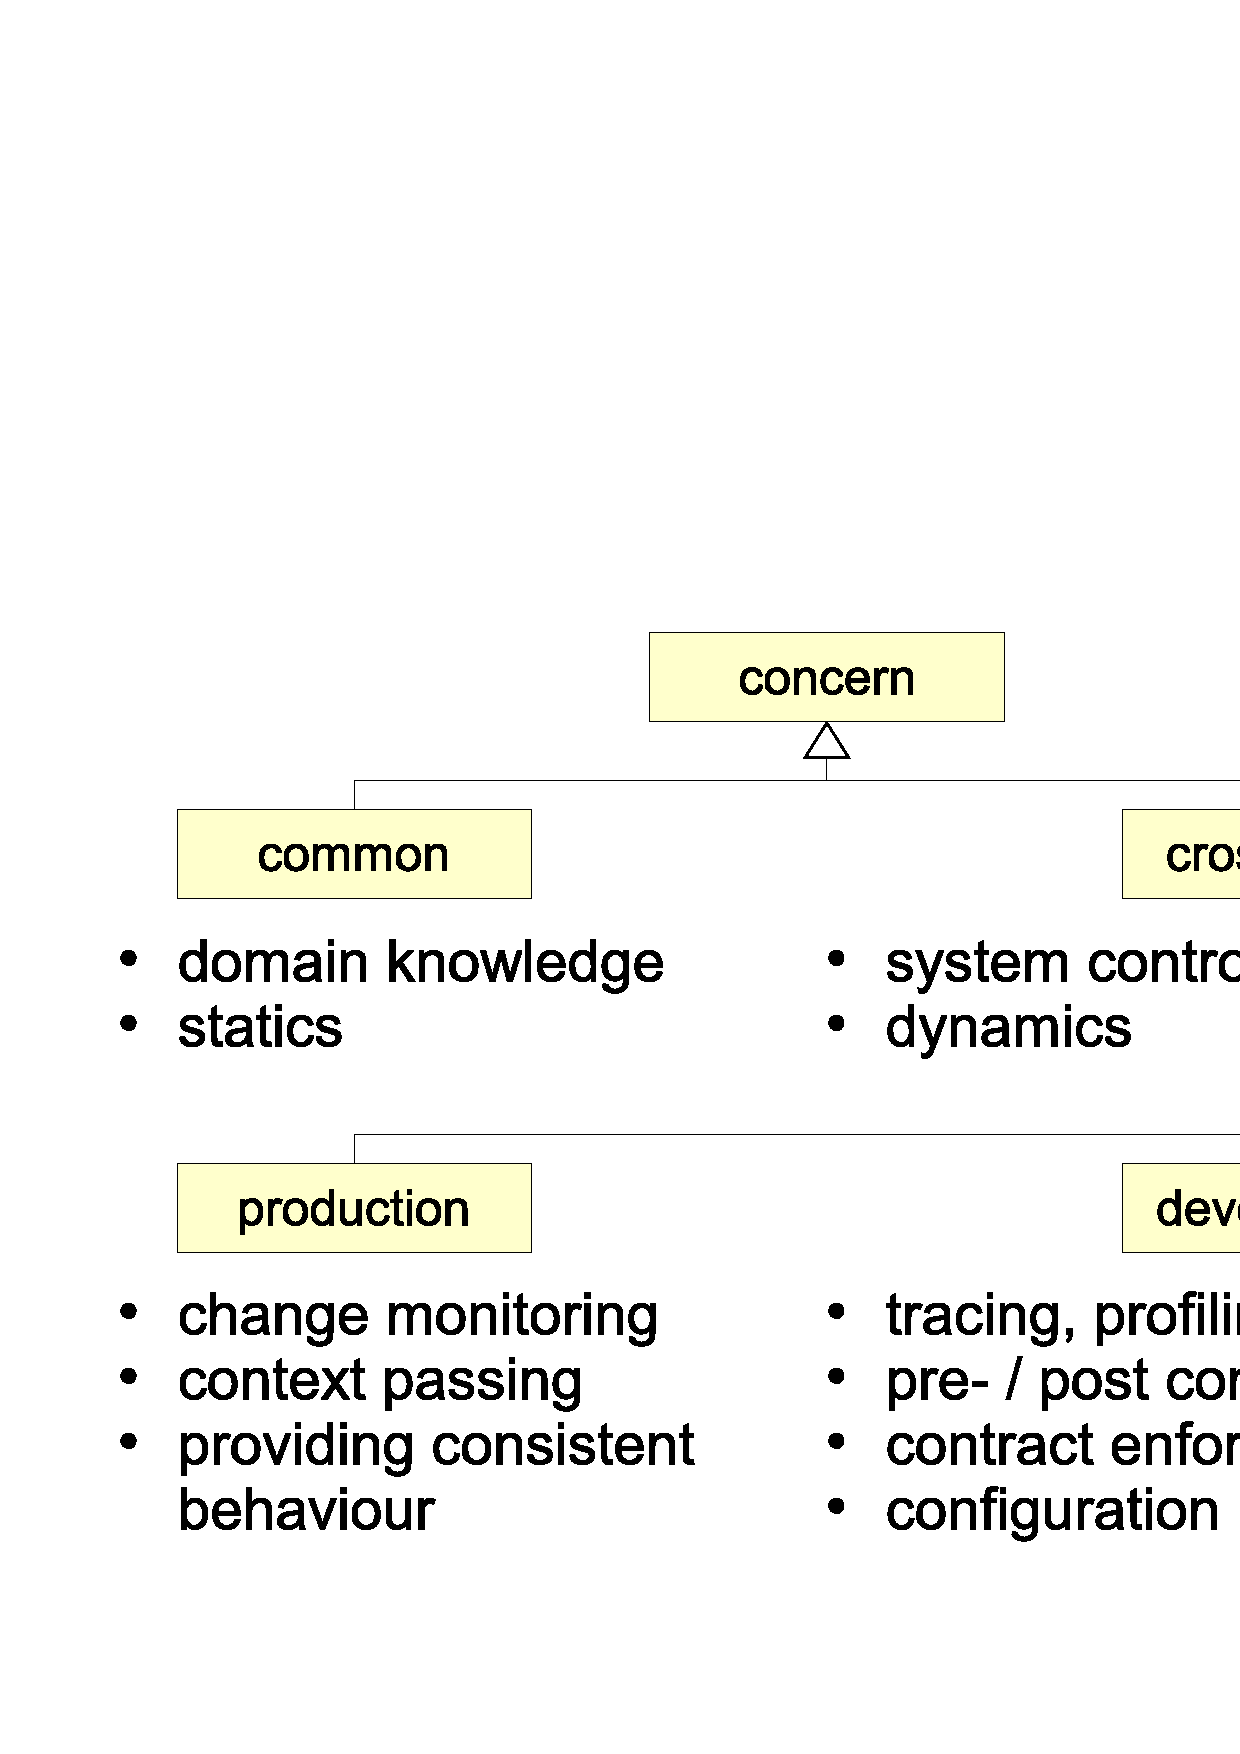
\includegraphics[scale=0.3,angle=-90]{graphic/concerns.pdf}
        \caption{Classification of Concerns}
        \label{concerns_figure}
    \end{center}
\end{figure}

Looking closer at these, it becomes obvious that crosscutting concerns represent
general \emph{System Control} functionality, while common concerns stand for
properties specific to an \emph{Application}. Comparing with nature (section
\ref{virtual_and_real_world_heading}), the separation of both kinds of concerns
seems absolutely correct. It arises the question, however, if AOP with all its
additional concepts is really the most suitable way for treating crosscutting
concerns? This work means \emph{no} and suggests to simply put all general
control functionality into a basic knowledge-interpreter system underlying all
applications (chapter \ref{cybernetics_oriented_interpreter_heading}).

%
% $RCSfile$
%
% Copyright (c) 2005-2006. Christian Heller. All rights reserved.
%
% Permission is granted to copy, distribute and/or modify this document
% under the terms of the GNU Free Documentation License, Version 1.1 or
% any later version published by the Free Software Foundation; with no
% Invariant Sections, with no Front-Cover Texts and with no Back-Cover
% Texts. A copy of the license is included in the section entitled
% "GNU Free Documentation License".
%
% http://www.cybop.net
% - Cybernetics Oriented Programming -
%
% http://www.resmedicinae.org
% - Information in Medicine -
%
% Version: $Revision$ $Date$ $Author$
% Authors: Christian Heller <christian.heller@tuxtax.de>
%

\subsubsection{Application and Domain}
\label{application_and_domain_heading}

Over the years, it has turned out to be helpful in software design, to separate
\emph{Domain Knowledge} from \emph{Application Functionality}. In
one-or-another form, the architectural software patterns \cite{heller2005}
\emph{Layers}, \emph{Domain Model} and \emph{Model View Controller} (MVC) all
suggest to apply this principle.

The \emph{Tools \& Materials} approach \cite{tandm} talks of \emph{active}
applications (tools) working on \emph{passive} domain data (material). And also
\emph{System Family Engineering} \cite{domainengg} bases on a separate
treatment of domain and application, in form of \emph{Domain Engineering} (DE)
and \emph{Application Engineering} (AE).

An often neglected fact of these approaches is that not only the domain, but
also the application contains important business knowledge (figure
\ref{separation_figure}). The \emph{User Interface} (UI), for example, is
tailored for a specific business domain. And the logic behind, if not
contained in the UI itself, is often put in a \emph{Controller} which belongs
to the application$-$, not the domain layer.

\begin{figure}[ht]
    \begin{center}
        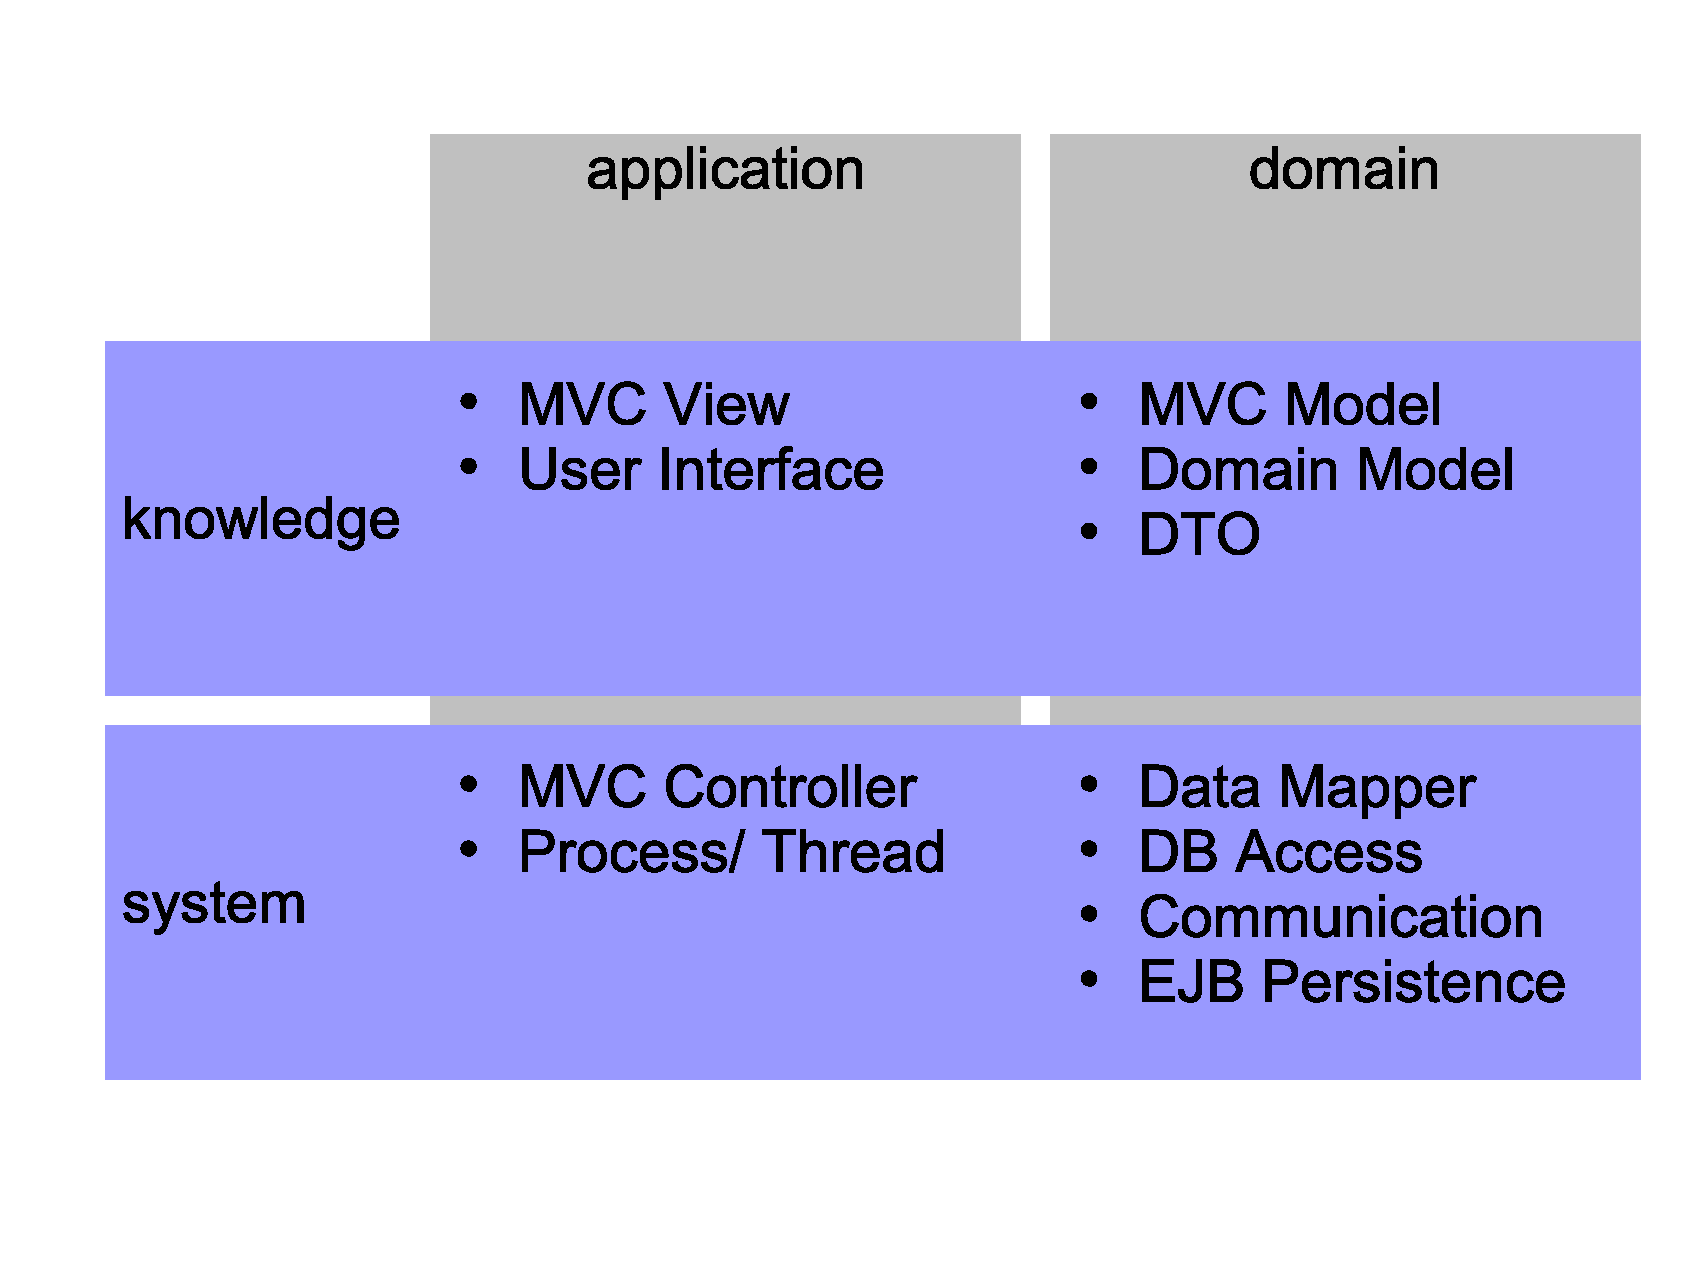
\includegraphics[scale=0.2]{vector/separation.eps}
        \caption{Different Knowledge Separations}
        \label{separation_figure}
    \end{center}
\end{figure}

Similarly, the domain often contains functionality which actually does belong
into the application process: \emph{Database} (DB) access is handled by help of
patterns like the \emph{Data Mapper} \cite{heller2005}, in which the mapper\\
objects contain \emph{Structured Query Language} (SQL) code to connect to a
\emph{Database Management System} (DBMS); \emph{Enterprise Java Beans} (EJB),
which should better be pure domain objects, imitate a \emph{Middleware}
providing persistence- or communication mechanisms, which originally have
nothing to do with the business knowledge they contain.

It is precisely this \emph{Mixup} of responsibilities between an application
system and its domain knowledge, that leads to multiple inter-dependencies and
hence unflexibility within a system. Instead, a separation should be made
between active \emph{System Control} and passive \emph{Knowledge}. A UI's
appearance would then be treated as domain knowledge, just as the logic of the
functions called through it. A data mapper would be transformed into a simple
\emph{Translator} -- similar to a \emph{Data Transfer Object} (DTO)
\cite{heller2005} -- that knows how to convert data from one domain model into
another; its DBMS access functionality, however, would be extracted and put
into the application system. Monstrosities like EJBs would likewise be opened
up and parted into their actual domain knowledge, and all other mechanisms
around -- the latter being moved into the application system.

To sum up this thought: The essential realisation here is that hardware-close
mechanisms like the ones necessary for data input/ output (i/o), enabling
inter-system communication, should be handled in an active application system
layer which was started as process on a computer, and \emph{not} be merged with
pure, passive domain knowledge. User interfaces and application logic which are
traditionally held in controller objects of the application layer, as well as
further business data models, should rather belong to a high-level knowledge
layer.

%
% $RCSfile$
%
% Copyright (c) 2002-2006. Christian Heller. All rights reserved.
%
% Permission is granted to copy, distribute and/or modify this document
% under the terms of the GNU Free Documentation License, Version 1.1 or
% any later version published by the Free Software Foundation; with no
% Invariant Sections, with no Front-Cover Texts and with no Back-Cover
% Texts. A copy of the license is included in the section entitled
% "GNU Free Documentation License".
%
% http://www.cybop.net
% - Cybernetics Oriented Programming -
%
% http://www.resmedicinae.org
% - Information in Medicine -
%
% Version: $Revision$ $Date$ $Author$
% Authors: Christian Heller <christian.heller@tuxtax.de>
%

\subsubsection{Platform Specific and -Independent}
\label{platform_specific_and_independent_heading}

The \emph{Model Driven Architecture} (MDA) \cite{mda} took a first step into
the right direction, by distinguishing \emph{Platform Independent Models}
(PIM), that is domain- and application logic, and \emph{Platform Specific Models}
(PSM), that is implementation technology. It encourages the use of automated
tools for defining and transforming these models.

While the definition, organisation and management of architectures (PIM) mostly
happen in the analysis- and design phase of a \emph{Software Engineering Process}
(SEP) (section \ref{abstraction_gaps_heading}), the generation of source code
(PSM) can be assigned to the implementation phase. The approach still has
weaknesses, and tools which can truly generate running systems are rare or not
existent, at least to what concerns more complex software systems -- not to
talk of the so-called \emph{Roundtrip Engineering}, which is managed by even
less tools.

Nevertheless, the trend clearly goes towards more model-centric approaches. The
aim of this work was to supply domain experts and application developers with a
\emph{Model Only} technology, allowing to create application systems that do
\emph{not} have to be transformed into classical implementation code any longer,
whereby the SEP abstraction gap number \emph{2} (figure \ref{gaps_figure})
could be closed conclusively. The knowledge schema introduced in section
\ref{knowledge_schema_heading} is a necessary prerequisite therefor.

%\input{kernel_and_user_mode}
%
% $RCSfile: agent_with_mental_state.tex,v $
%
% Copyright (C) 2002-2008. Christian Heller.
%
% Permission is granted to copy, distribute and/or modify this document
% under the terms of the GNU Free Documentation License, Version 1.1 or
% any later version published by the Free Software Foundation; with no
% Invariant Sections, with no Front-Cover Texts and with no Back-Cover
% Texts. A copy of the license is included in the section entitled
% "GNU Free Documentation License".
%
% http://www.cybop.net
% - Cybernetics Oriented Programming -
%
% http://www.resmedicinae.org
% - Information in Medicine -
%
% Version: $Revision: 1.1 $ $Date: 2008-08-19 20:41:05 $ $Author: christian $
% Authors: Christian Heller <christian.heller@tuxtax.de>
%

\subsection{Agent with Mental State}
\label{agent_with_mental_state_heading}
\index{Agent Oriented Programming}
\index{AGOP}
\index{Agent}
\index{Mental State of an Agent}
\index{Formal Knowledge Representation Language of AGOP}
\index{Agent Programming Language of AGOP}
\index{Conversion Method of AGOP}

One design paradigm that early recognised the advantages of splitting software
into low-level system control and high-level knowledge, is
\emph{Agent Oriented Programming} (AGOP) (section
\ref{agent_oriented_programming_heading}). \emph{Agents}, as active software
components (which in this work means: \emph{running in an own process}), have
a \emph{Mental State} representing their knowledge, which they are able to
interpret and manipulate. This approach was copied in CYBOP.

Of the three elements \emph{Formal Knowledge Representation Language},
\emph{Agent Programming Language} and \emph{Conversion Method}, which an AGOP
system, after section \ref{agent_oriented_programming_heading}, needs in order
to be complete, this work provides the first two in form of the
\emph{Cybernetics Oriented Language} (CYBOL) and the
\emph{Cybernetics Oriented Interpreter} (CYBOI), described in sections
\ref{cybernetics_oriented_language_heading} and
\ref{cybernetics_oriented_interpreter_heading}, respectively. Thereby, CYBOI
itself is not a language, but represents a ready system, written in the
\emph{C} programming language. A method for converting traditional applications
into agents is not provided, since methodologies are clearly \emph{not} a topic
of this work.

Of course, there are differences distinguishing
\emph{Cybernetics Oriented Programming} (CYBOP) from traditional AGOP systems.
CYBOP needs an own interpreter, because of its new knowledge representation
philosophy and -language, which are the topic of chapters
\ref{knowledge_schema_heading} and \ref{cybernetics_oriented_language_heading}.
One reason for the difficult handling and intransparency of many traditional
knowledge representation languages is that they mix two kinds of knowledge:
\emph{State-} and \emph{Logic} descriptions. More on how this is avoided in
CYBOP in chapter \ref{state_and_logic_heading}.

One may wonder why such a supposedly advantageous architecture is not used by
all of today's systems? One reason may be that AGOP is still a rather young
technology lacking the necessary popularity. Another reason may be the bad
reputation of AGOP systems (and just about everything that has to do with
knowledge representation) among average developers -- partly because of their
immaturity, but mostly because of their complicated knowledge models and
-handling. Looking at the often quite cryptic appearance of the corresponding
languages, one tends to understand the developers' dislike.

%
% $RCSfile$
%
% Copyright (c) 2005-2006. Christian Heller. All rights reserved.
%
% Permission is granted to copy, distribute and/or modify this document
% under the terms of the GNU Free Documentation License, Version 1.1 or
% any later version published by the Free Software Foundation; with no
% Invariant Sections, with no Front-Cover Texts and with no Back-Cover
% Texts. A copy of the license is included in the section entitled
% "GNU Free Documentation License".
%
% http://www.cybop.net
% - Cybernetics Oriented Programming -
%
% http://www.resmedicinae.org
% - Information in Medicine -
%
% Version: $Revision$ $Date$ $Author$
% Authors: Christian Heller <christian.heller@tuxtax.de>
%

\subsubsection{Data Garden}
\label{data_garden_heading}

Now, if a distinction of high-level knowledge from low-level system control
software is considered to be useful, the next question must be: \textit{How,
that is in which form, best to store knowledge in a system?}

One possible structure called \emph{Data Garden} \cite{holland} was proposed by
Wau Holland of the \emph{Chaos Computer Club} (CCC). Although being a
non-academic organisation, his ideas on knowledge modelling are interesting to
this work. He dreamt of whole \emph{Forests}, \emph{Parks} or -- as the name
says -- \emph{Gardens} of \emph{Knowledge Trees} and \emph{Data Bushes} (figure
\ref{garden_figure}).

\begin{figure}[ht]
    \begin{center}
        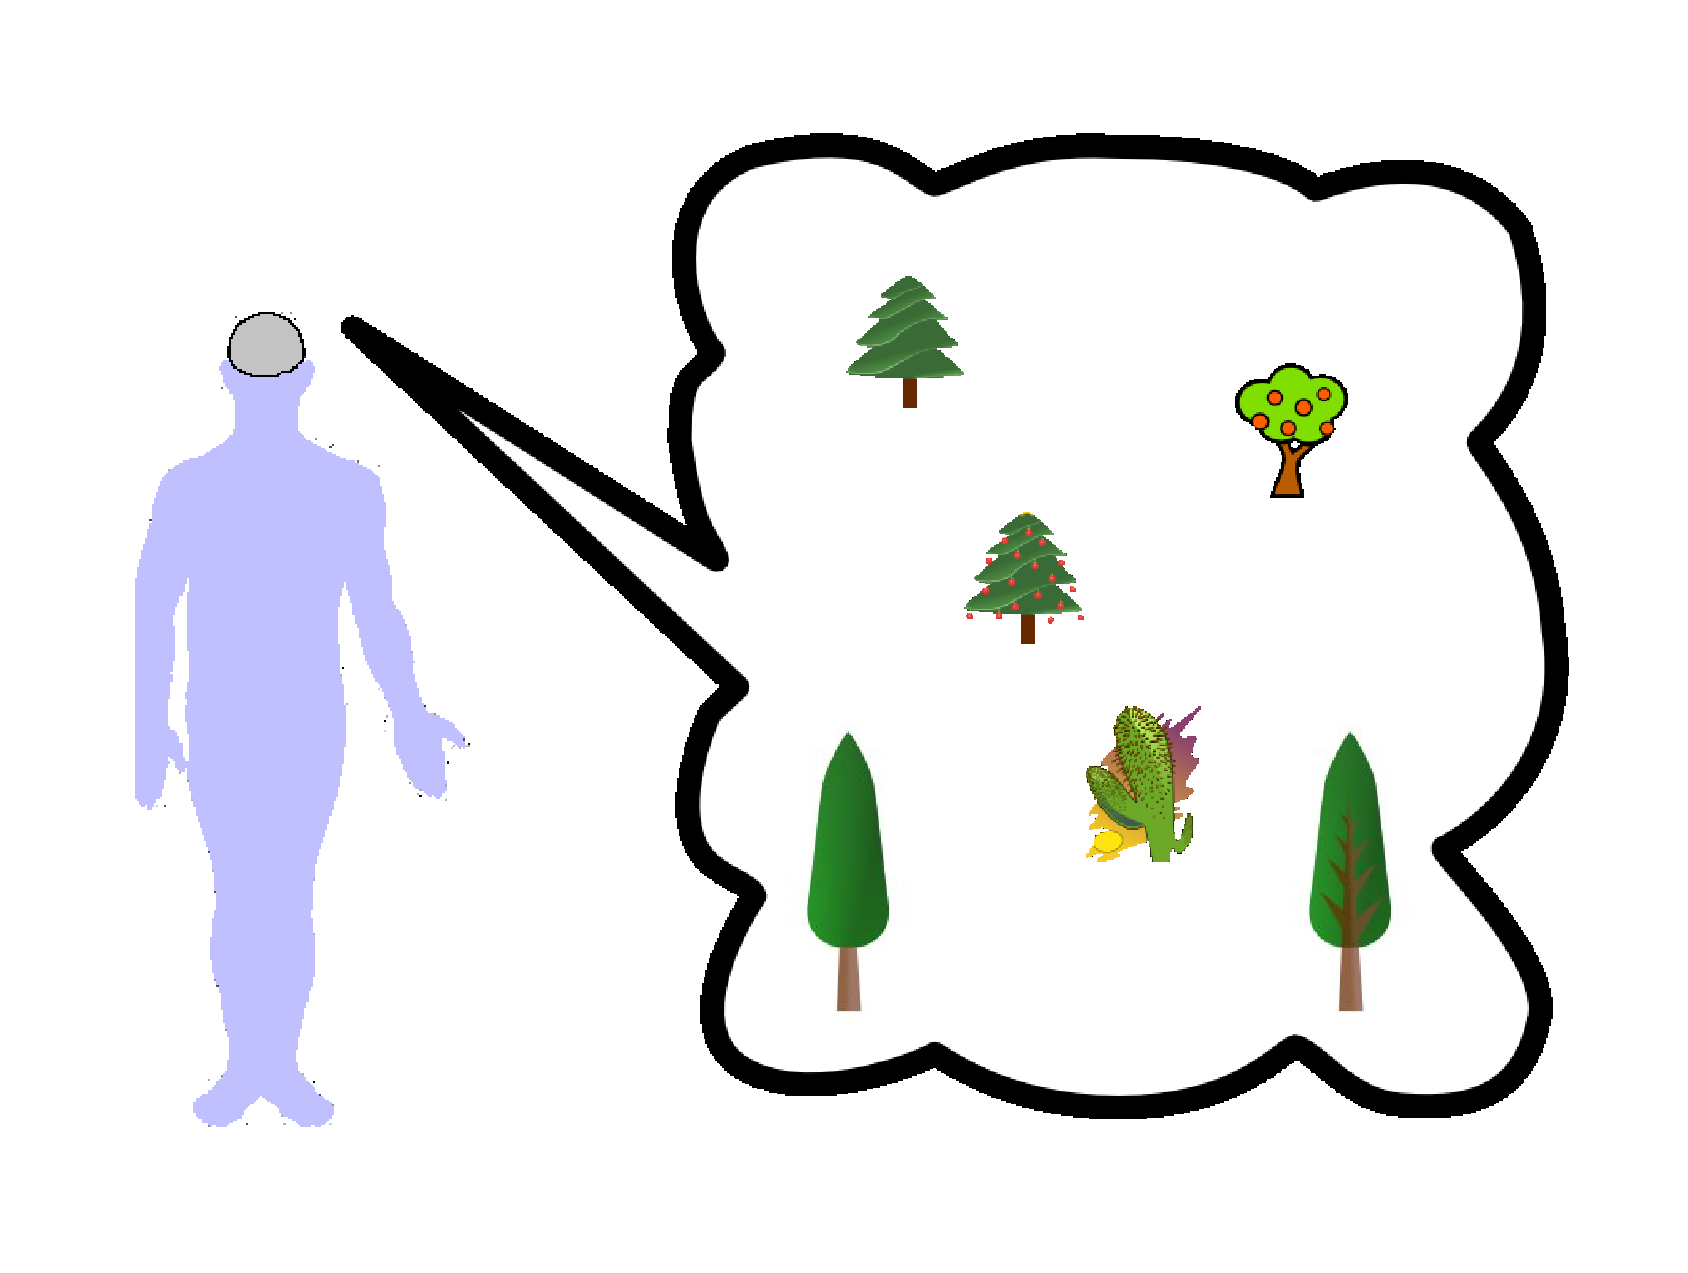
\includegraphics[scale=0.2]{vector/garden.eps}
        \caption{Data Garden}
        \label{garden_figure}
    \end{center}
\end{figure}

The interpreter (section \ref{cyboi_heading}) created in the work described in
this article stores all its knowledge in \emph{one single} tree, whose root
node it references. The single concepts (data bushes) are represented by
branches of that knowledge tree.

